\documentclass[11pt]{beamer}
% \usetheme{Boadilla}
  \usetheme{default}


% acronyms for text or math mode
\newcommand {\ccast} {\mbox{\small CCAST}}
\newcommand {\cris} {\mbox{\small CrIS}}

\newcommand {\airs} {\mbox{\small AIRS}}
\newcommand {\iasi} {\mbox{\small IASI}}
\newcommand {\idps} {\mbox{\small IDPS}}
\newcommand {\nasa} {\mbox{\small NASA}}
\newcommand {\noaa} {\mbox{\small NOAA}}
\newcommand {\nstar} {\mbox{\small STAR}}
\newcommand {\umbc} {\mbox{\small UMBC}}
\newcommand {\uw}   {\mbox{\small UW}}

\newcommand {\fft}  {\mbox{\small FFT}}
\newcommand {\ifft} {\mbox{\small IFFT}}
\newcommand {\fir}  {\mbox{\small FIR}}
\newcommand {\fov}  {\mbox{\small FOV}}
\newcommand {\for}  {\mbox{\small FOR}}
\newcommand {\ict}  {\mbox{\small ICT}}
\newcommand {\ils}  {\mbox{\small ILS}}
\newcommand {\igm}  {\mbox{\small IGM}}
\newcommand {\opd}  {\mbox{\small OPD}}
\newcommand {\rms}  {\mbox{\small RMS}}
\newcommand {\zpd}  {\mbox{\small ZPD}}
\newcommand {\ppm}  {\mbox{\small PPM}}
\newcommand {\srf}  {\mbox{\small SRF}}

\newcommand {\ES} {\mbox{\small ES}}
\newcommand {\SP} {\mbox{\small SP}}
\newcommand {\IT} {\mbox{\small IT}}
\newcommand {\SA} {\mbox{\small SA}}

\newcommand {\ET} {\mbox{\small ET}}
\newcommand {\FT} {\mbox{\small FT}}

% abbreviations, mainly for math mode
\newcommand {\real} {\mbox{real}}
\newcommand {\imag} {\mbox{imag}}
\newcommand {\atan} {\mbox{atan}}
\newcommand {\obs}  {\mbox{obs}}
\newcommand {\calc} {\mbox{calc}}
\newcommand {\sinc} {\mbox{sinc}}
\newcommand {\psinc} {\mbox{psinc}}
\newcommand {\std} {\mbox{std}}

% symbols, for math mode only
\newcommand {\wnum} {\mbox{cm$^{-1}$}}
\newcommand {\lmax} {L_{\mbox{\tiny max}}}
\newcommand {\vmax} {V_{\mbox{\tiny max}}}

\newcommand {\tauobs} {\tau_{\mbox{\tiny obs}}}
\newcommand {\taucal} {\tau_{\mbox{\tiny calc}}}
\newcommand {\Vdc}  {V_{\mbox{\tiny DC}}}

\newcommand {\rIT} {r_{\mbox{\tiny\textsc{ict}}}}
\newcommand {\rES} {r_{\mbox{\tiny\textsc{es}}}}
\newcommand {\robs} {r_{\mbox{\tiny obs}}}

\newcommand {\rITobs} {r_{\mbox{\tiny\textsc{ict}}}^{\mbox{\tiny obs}}}
\newcommand {\rITcal} {r_{\mbox{\tiny\textsc{ict}}}^{\mbox{\tiny cal}}}

\newcommand {\ITmean} {\langle\mbox{\small IT}\rangle}
\newcommand {\SPmean} {\langle\mbox{\small SP}\rangle}


\title{CrIS Calibration Equations}
\author{H.~E.~Motteler and L.~L.~Strow}
\institute{
  UMBC Atmospheric Spectroscopy Lab \\
  Joint Center for Earth Systems Technology \\
}
\date{\today}
\begin{document}

%----------- slide --------------------------------------------------%
\begin{frame}[plain]
\titlepage
\end{frame}
%----------- slide --------------------------------------------------%
\begin{frame}
\frametitle{SW high res psinc ILS}

\begin{center}
  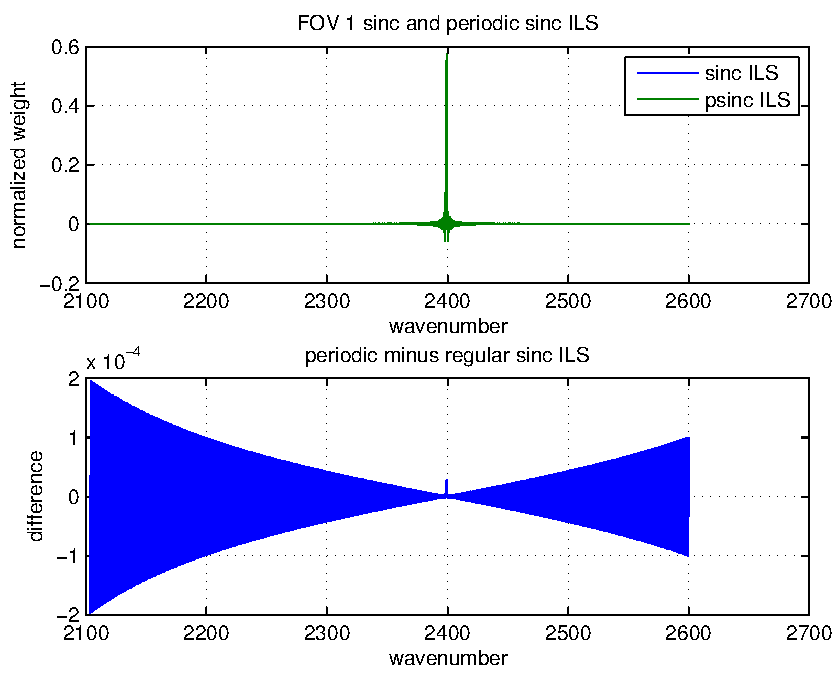
\includegraphics[scale=0.6]{figures/psinc_hires2.pdf}
\end{center}

\end{frame}
%----------- slide --------------------------------------------------%
\begin{frame}
\frametitle{SW low res psinc ILS}

\begin{center}
  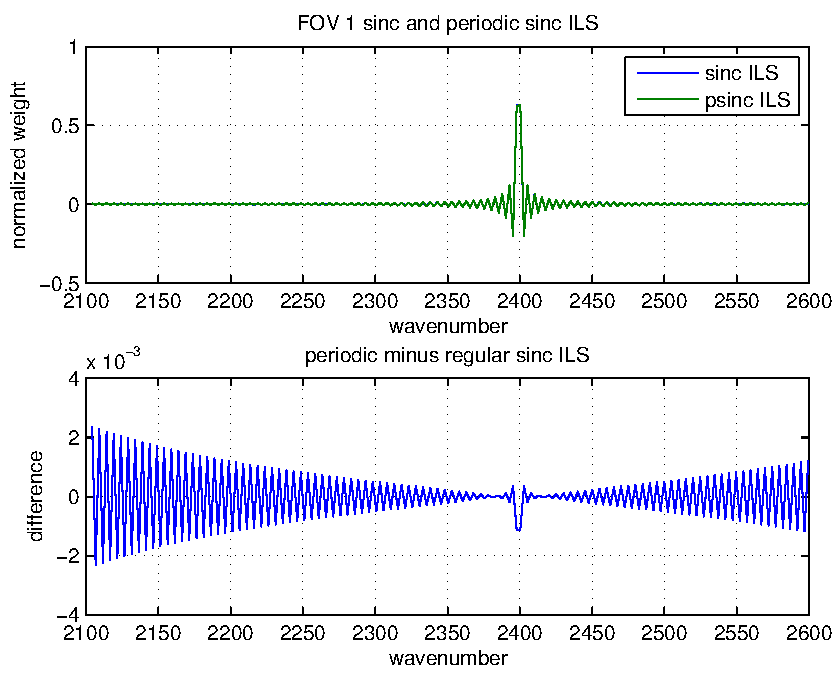
\includegraphics[scale=0.6]{figures/psinc_lowres.pdf}
\end{center}

\end{frame}
%----------- slide --------------------------------------------------%
\begin{frame}
\frametitle{basic functions}

\begin{itemize}
  \item unnormalized sinc, $\sinc(x) = \sin(x) / x$
  \item unnormalized periodic sinc, 
    $\psinc(x, n) = \sin(x) / (n \cdot\sin(x/n))$
  \item NEED ILS
\end{itemize}

\end{frame}
%----------- slide --------------------------------------------------%
\begin{frame}
\frametitle{methods}

The main processing steps are

\begin{itemize}
  \item read the CCSDS data packets
  \item take interferograms to count spectra
  \item take the mean of spectra over stable test intervals
  \item find $\tauobs = f\circ\SA^{-1}\circ f((\FT_2 - \FT_1) / (\ET_2 - \ET_1))$
  \item compare observed and calculated spectra
\end{itemize}

The last step can be embedded in a search where we minimize
$\rms(a\cdot\tauobs + b - \taucal)$ as a function of metrology laser
wavelength.  From this we get both a conventional residual and the
difference of wavelength at the minima from the Neon calibration
value.

\end{frame}
%----------- slide --------------------------------------------------%
\begin{frame}
\frametitle{applications}

\begin{itemize}
  \item gas cell tests may help resolve questions about the best
    form of the ILS and calibration equations.

  \item we have both good calculated data and observations averaged
    over many looks.  But the spectral signal is small relative to
    the BB as seen thru the filters, and not always larger than the
    obs to obs variance.

  \item our initial tests found no significant difference in
    periodic vs regular sinc in compairing obs minus calc or sweep
    directions.

  \item we did see a 1 or 2 PPM improvement in the metrology laser
    residuals with a calibration equation of the form
    \[\tauobs = f(\SA^{-1}f(\FT_2 - \FT_1) / \SA^{-1}f(\ET_2 - \ET_1)) \]

\end{itemize}

\end{frame}
%----------- slide --------------------------------------------------%
\end{document}
